\documentclass[ignorenonframetext,t]{beamer}
\setbeamertemplate{caption}[numbered]
\setbeamertemplate{caption label separator}{: }
\setbeamercolor{caption name}{fg=normal text.fg}
\beamertemplatenavigationsymbolsempty
\usepackage{lmodern}
\usepackage{amssymb,amsmath}
\usepackage{ifxetex,ifluatex}
\usepackage{fixltx2e} % provides \textsubscript
\ifnum 0\ifxetex 1\fi\ifluatex 1\fi=0 % if pdftex
  \usepackage[T1]{fontenc}
  \usepackage[utf8]{inputenc}
\else % if luatex or xelatex
  \ifxetex
    \usepackage{mathspec}
  \else
    \usepackage{fontspec}
  \fi
  \defaultfontfeatures{Ligatures=TeX,Scale=MatchLowercase}
\fi
\usecolortheme{spruce}
\usefonttheme{serif}
% use upquote if available, for straight quotes in verbatim environments
\IfFileExists{upquote.sty}{\usepackage{upquote}}{}
% use microtype if available
\IfFileExists{microtype.sty}{%
\usepackage{microtype}
\UseMicrotypeSet[protrusion]{basicmath} % disable protrusion for tt fonts
}{}
\newif\ifbibliography
\hypersetup{
            pdftitle={Week 6: Graphical Data Exploration},
            colorlinks=true,
            linkcolor=Maroon,
            citecolor=Blue,
            urlcolor=blue,
            breaklinks=true}
\urlstyle{same}  % don't use monospace font for urls
\usepackage{color}
\usepackage{fancyvrb}
\newcommand{\VerbBar}{|}
\newcommand{\VERB}{\Verb[commandchars=\\\{\}]}
\DefineVerbatimEnvironment{Highlighting}{Verbatim}{commandchars=\\\{\}}
% Add ',fontsize=\small' for more characters per line
\usepackage{framed}
\definecolor{shadecolor}{RGB}{248,248,248}
\newenvironment{Shaded}{\begin{snugshade}}{\end{snugshade}}
\newcommand{\KeywordTok}[1]{\textcolor[rgb]{0.13,0.29,0.53}{\textbf{#1}}}
\newcommand{\DataTypeTok}[1]{\textcolor[rgb]{0.13,0.29,0.53}{#1}}
\newcommand{\DecValTok}[1]{\textcolor[rgb]{0.00,0.00,0.81}{#1}}
\newcommand{\BaseNTok}[1]{\textcolor[rgb]{0.00,0.00,0.81}{#1}}
\newcommand{\FloatTok}[1]{\textcolor[rgb]{0.00,0.00,0.81}{#1}}
\newcommand{\ConstantTok}[1]{\textcolor[rgb]{0.00,0.00,0.00}{#1}}
\newcommand{\CharTok}[1]{\textcolor[rgb]{0.31,0.60,0.02}{#1}}
\newcommand{\SpecialCharTok}[1]{\textcolor[rgb]{0.00,0.00,0.00}{#1}}
\newcommand{\StringTok}[1]{\textcolor[rgb]{0.31,0.60,0.02}{#1}}
\newcommand{\VerbatimStringTok}[1]{\textcolor[rgb]{0.31,0.60,0.02}{#1}}
\newcommand{\SpecialStringTok}[1]{\textcolor[rgb]{0.31,0.60,0.02}{#1}}
\newcommand{\ImportTok}[1]{#1}
\newcommand{\CommentTok}[1]{\textcolor[rgb]{0.56,0.35,0.01}{\textit{#1}}}
\newcommand{\DocumentationTok}[1]{\textcolor[rgb]{0.56,0.35,0.01}{\textbf{\textit{#1}}}}
\newcommand{\AnnotationTok}[1]{\textcolor[rgb]{0.56,0.35,0.01}{\textbf{\textit{#1}}}}
\newcommand{\CommentVarTok}[1]{\textcolor[rgb]{0.56,0.35,0.01}{\textbf{\textit{#1}}}}
\newcommand{\OtherTok}[1]{\textcolor[rgb]{0.56,0.35,0.01}{#1}}
\newcommand{\FunctionTok}[1]{\textcolor[rgb]{0.00,0.00,0.00}{#1}}
\newcommand{\VariableTok}[1]{\textcolor[rgb]{0.00,0.00,0.00}{#1}}
\newcommand{\ControlFlowTok}[1]{\textcolor[rgb]{0.13,0.29,0.53}{\textbf{#1}}}
\newcommand{\OperatorTok}[1]{\textcolor[rgb]{0.81,0.36,0.00}{\textbf{#1}}}
\newcommand{\BuiltInTok}[1]{#1}
\newcommand{\ExtensionTok}[1]{#1}
\newcommand{\PreprocessorTok}[1]{\textcolor[rgb]{0.56,0.35,0.01}{\textit{#1}}}
\newcommand{\AttributeTok}[1]{\textcolor[rgb]{0.77,0.63,0.00}{#1}}
\newcommand{\RegionMarkerTok}[1]{#1}
\newcommand{\InformationTok}[1]{\textcolor[rgb]{0.56,0.35,0.01}{\textbf{\textit{#1}}}}
\newcommand{\WarningTok}[1]{\textcolor[rgb]{0.56,0.35,0.01}{\textbf{\textit{#1}}}}
\newcommand{\AlertTok}[1]{\textcolor[rgb]{0.94,0.16,0.16}{#1}}
\newcommand{\ErrorTok}[1]{\textcolor[rgb]{0.64,0.00,0.00}{\textbf{#1}}}
\newcommand{\NormalTok}[1]{#1}
\usepackage{longtable,booktabs}
\usepackage{caption}
% These lines are needed to make table captions work with longtable:
\makeatletter
\def\fnum@table{\tablename~\thetable}
\makeatother

% Prevent slide breaks in the middle of a paragraph:
\widowpenalties 1 10000
\raggedbottom

\AtBeginPart{
  \let\insertpartnumber\relax
  \let\partname\relax
  \frame{\partpage}
}
\AtBeginSection{
  \ifbibliography
  \else
    \let\insertsectionnumber\relax
    \let\sectionname\relax
    \frame{\sectionpage}
  \fi
}
\AtBeginSubsection{
  \let\insertsubsectionnumber\relax
  \let\subsectionname\relax
  \frame{\subsectionpage}
}

\setlength{\parindent}{0pt}
\setlength{\parskip}{6pt plus 2pt minus 1pt}
\setlength{\emergencystretch}{3em}  % prevent overfull lines
\providecommand{\tightlist}{%
  \setlength{\itemsep}{0pt}\setlength{\parskip}{0pt}}
\setcounter{secnumdepth}{0}
\usepackage{multicol}
\usepackage{tikz}
\usepackage{tikzpagenodes}
\definecolor{grn}{rgb}{0.0, 0.2, 0.0}
\usepackage{tabto}
\usepackage{verbatim}
\usepackage{amsmath}
\usepackage{mathtools}
\usepackage{graphicx}
\definecolor{OG}{RGB}{0,64,8}
\definecolor{LG}{RGB}{0,102,51}
\definecolor{myRed}{RGB}{228,26,28}
\definecolor{myBlue}{RGB}{55,126,184}
\definecolor{myGreen}{RGB}{77,175,74}
\definecolor{myPurple}{RGB}{152,78,163}
\setbeamercolor{itemize item}{fg=white!0!LG}
\setbeamercolor{enumerate item}{fg=white!0!LG}
\setbeamercolor{enumerate subitem}{fg=white!70!LG}
\setbeamercolor{itemize subitem}{fg=white!70!LG}
\setbeamercolor{itemize subsubitem}{fg=white!70!LG}
\setbeamercolor{navigation symbols}{fg=white!70!LG, bg=white!70!LG}
\usepackage{inputenc}
\usepackage{booktabs}
\usepackage{caption}
\usetikzlibrary{patterns,arrows,decorations.pathreplacing}

\title{Week 6: Graphical Data Exploration}
\subtitle{Session 1}
\date{Spring 2020}

\begin{document}
\frame{\titlepage}

\begin{frame}[fragile]{iClicker Question \textcolor{blue}{1}}

Which of the following should I use to read the file \texttt{mydata.csv}
into a data frame called \texttt{dat} in R?

\begin{enumerate}[A]
\item \texttt{dat = read.csv(mydata.csv)}
\item \texttt{read.csv(mydata.csv)}
\item \texttt{dat = read.csv("mydata.csv")}
\item \texttt{read.csv(mydata.csv, row.names = 1)}
\item \texttt{read.csv("mydata.csv")}
\end{enumerate}

\vfill

\begin{tikzpicture}[remember picture,overlay]
\node[xshift=-2cm,yshift=1cm] at (current page.south east)
{
\includegraphics[height=0.25in]{../slide_images/iClicker_logo.png}};
\end{tikzpicture}

\end{frame}

\begin{frame}{iClicker Question \textcolor{blue}{2}}

Which symbol do we use to represent the \textbf{sample mean}?

\begin{enumerate}[A]
\item $\sigma$
\item $\bar s$
\item $\bar{x}$
\item $\mu$
\item $\bar{m}$
\end{enumerate}

\vfill

\begin{tikzpicture}[remember picture,overlay]
\node[xshift=-2cm,yshift=1cm] at (current page.south east)
{
\includegraphics[height=0.25in]{iClicker_logo.png}};
\end{tikzpicture}

\end{frame}

\begin{frame}{iClicker Question \textcolor{blue}{3}}

Which symbol do we use to represent the \textbf{population mean}?

\begin{enumerate}[A]
\item $\sigma$
\item $\bar s$
\item $\bar{x}$
\item $\mu$
\item $\bar{m}$
\end{enumerate}

\vfill

\begin{tikzpicture}[remember picture,overlay]
\node[xshift=-2cm,yshift=1cm] at (current page.south east)
{
\includegraphics[height=0.25in]{../slide_images/iClicker_logo.png}};
\end{tikzpicture}

\end{frame}

\begin{frame}{iClicker Question \textcolor{blue}{4}}

Which plot type is most appropriate to show the \textbf{distribution} of
a set of measurements?

\begin{enumerate}[A]
\item scatterplot
\item boxplot
\item barchart
\item histogram
\item pie chart
\end{enumerate}

\vfill

\begin{tikzpicture}[remember picture,overlay]
\node[xshift=-2cm,yshift=1cm] at (current page.south east)
{
\includegraphics[height=0.25in]{../slide_images/iClicker_logo.png}};
\end{tikzpicture}

\end{frame}

\begin{frame}[fragile]{iClicker Question \textcolor{blue}{5}}

Which of the following lines of code will make a scatterplot of the
dataframe with length on the x-axis and mass on the y-axis?

\begin{verbatim}
##      length     width mass
## 1 0.7209039 2.8777226   37
## 2 0.8757732 1.6052823   29
## 3 0.7609823 0.4713699   19
\end{verbatim}

\begin{enumerate}[A]
\item \texttt{plot(dat\$mass, dat\$length)}
\item \texttt{scatter(dat\$length, dat\$mass)}
\item \texttt{boxplot(dat\$length, dat\$mass, type = "p")}
\item \texttt{dotplot(dat\$length, dat\$mass)}
\item \texttt{plot(dat\$length, dat\$mass)}
\end{enumerate}

\vfill

\begin{tikzpicture}[remember picture,overlay]
\node[xshift=-2cm,yshift=1cm] at (current page.south east)
{
\includegraphics[height=0.25in]{../slide_images/iClicker_logo.png}};
\end{tikzpicture}

\end{frame}

\begin{frame}{Announcements}

Trying a different slide layout today

\end{frame}

\begin{frame}{Graphical exploration}

Why use graphs?

\begin{tikzpicture}[remember picture,overlay]
\node[xshift=0cm,yshift=0cm] at (current page)
{
\includegraphics[height=2in]{C:/Users/michaelnelso/git/NRC290B/slides/slide_images/question_mark_green.png}};
\end{tikzpicture}

\end{frame}

\begin{frame}{Graphical exploration}

Two main reasons to use graphs:

\begin{itemize}
\item[1.]<1-> Inform how to analyze the data
  \begin{itemize}
  \item<2-> visualization
  \item<2-> identify patterns
  \item<2-> choose appropriate statistical test
  \end{itemize}
\item[2.]<1-> Presentation of the data
  \begin{itemize}
  \item<3-> summarize results
  \item<3-> communicate results
  \item<3-> publish results
  \end{itemize}
\end{itemize}

\begin{tikzpicture}[remember picture,overlay]
\node[xshift=0cm,yshift=-2.8cm] at (current page)
{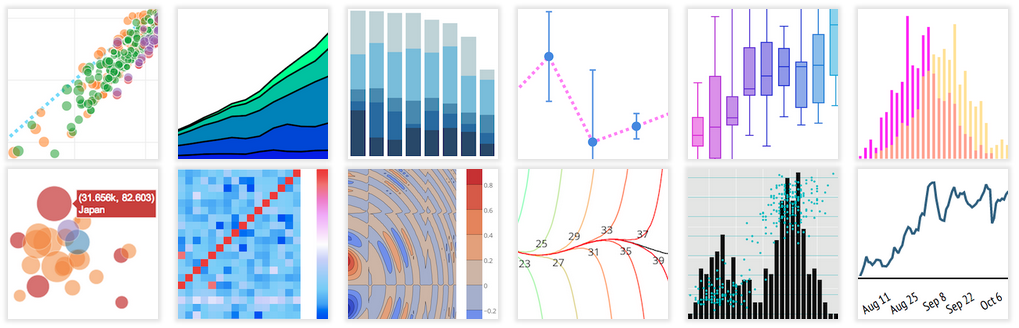
\includegraphics[height=1in]{C:/Users/michaelnelso/git/NRC290B/Images/graffs.png}};
\end{tikzpicture}

\end{frame}

\begin{frame}{Types of graphs - \emph{Exploratory}}

Exploratory graphs help understand the distribution of the data:

\begin{itemize}
\tightlist
\item
  are the data normally distributed

  \begin{itemize}
  \tightlist
  \item
    important assumption in statistics
  \item
    determines how data are analyzed
  \end{itemize}
\item
  what is the central tendency
\item
  what is the spread
\item
  general summaries of the data
\end{itemize}

\end{frame}

\begin{frame}[fragile]{Exploratory: \emph{Histogram}}

\begin{itemize}
\tightlist
\item
  width of bars are defined data bins or intervals
\item
  height of bars represent bin-specific frequencies
\end{itemize}

\begin{Shaded}
\begin{Highlighting}[]
\KeywordTok{hist}\NormalTok{(values)}
\end{Highlighting}
\end{Shaded}

\begin{tikzpicture}[remember picture,overlay]
\node[yshift=2cm] at (current page.south)
{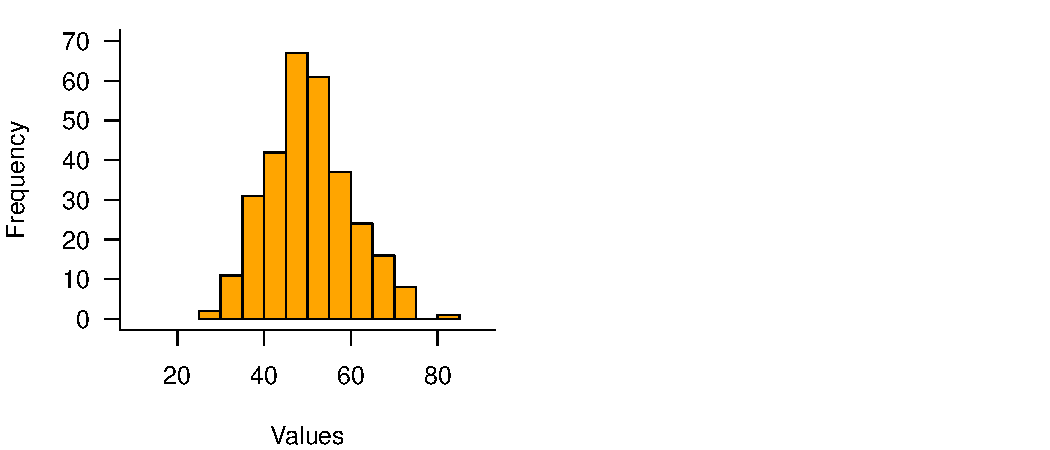
\includegraphics[height=1.9in]{C:/Users/michaelnelso/git/NRC290B/slides/slide_images/randhist.pdf}};
\end{tikzpicture}

\end{frame}

\begin{frame}[fragile]{Exploratory: \emph{Histogram}}

\begin{itemize}
\tightlist
\item
  width of bars are defined data bins or intervals
\item
  height of bars represent bin-specific frequencies
\end{itemize}

You can change the number and widths of the bins.

\begin{Shaded}
\begin{Highlighting}[]
\KeywordTok{hist}\NormalTok{(values, }\DataTypeTok{breaks=}\KeywordTok{seq}\NormalTok{(}\DecValTok{10}\NormalTok{,}\DecValTok{90}\NormalTok{,}\DecValTok{2}\NormalTok{))}
\end{Highlighting}
\end{Shaded}

\begin{tikzpicture}[remember picture,overlay]
\node[yshift=2cm] at (current page.south)
{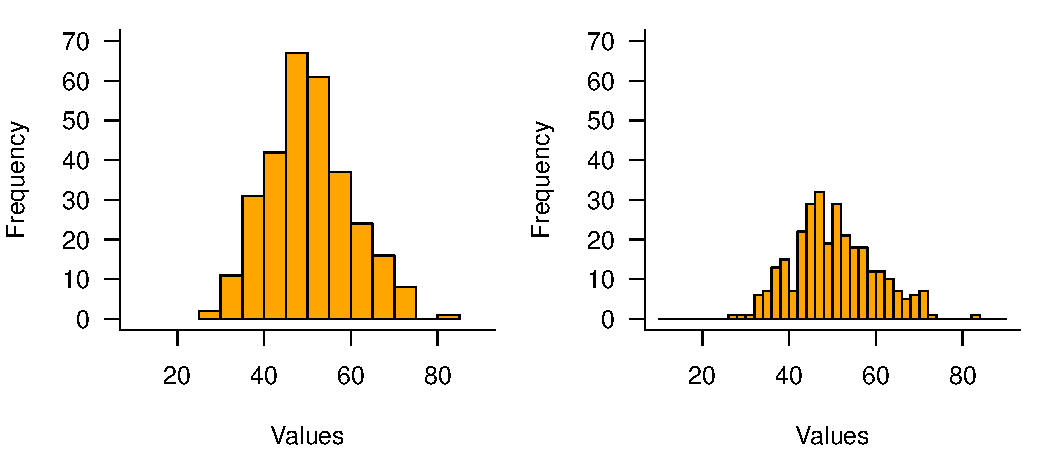
\includegraphics[height=1.9in]{C:/Users/michaelnelso/git/NRC290B/slides/slide_images/randhist2.pdf}};
\end{tikzpicture}

\end{frame}

\begin{frame}[fragile]{Exploratory: \emph{Histogram + Density Plot}}

A \emph{density plot}: smoothed version of histogram

\begin{itemize}
\tightlist
\item
  To overlay on a histogram, tell \texttt{hist()} to plot the
  \emph{probability} version of the histogram:
\end{itemize}

\begin{Shaded}
\begin{Highlighting}[]
\KeywordTok{hist}\NormalTok{(values, }\DataTypeTok{probability=}\OtherTok{TRUE}\NormalTok{)}
\KeywordTok{lines}\NormalTok{(}\KeywordTok{density}\NormalTok{(values))}
\end{Highlighting}
\end{Shaded}

\begin{tikzpicture}[remember picture,overlay]
\node[yshift=2cm] at (current page.south)
{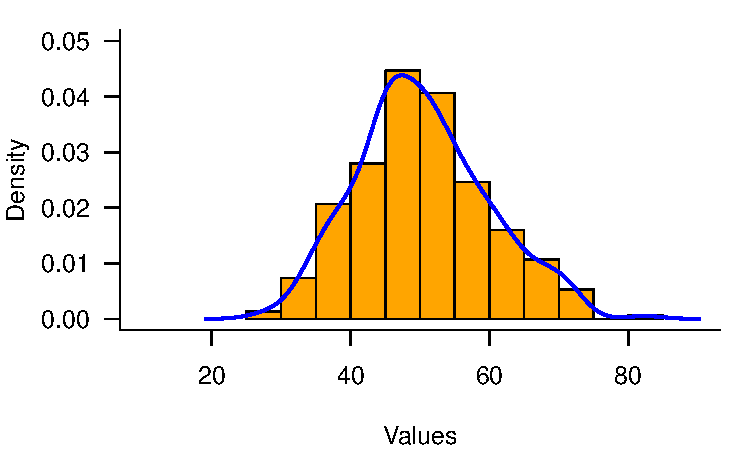
\includegraphics[height=1.9in]{C:/Users/michaelnelso/git/NRC290B/slides/slide_images/randhist3.pdf}};
\end{tikzpicture}

\end{frame}

\begin{frame}[fragile]{Exploratory: \emph{Box-whisker/Box plot}}

\begin{itemize}
\tightlist
\item
  distribution
\item
  outliers
\item
  symmetry or skewness
\end{itemize}

\begin{Shaded}
\begin{Highlighting}[]
\KeywordTok{boxplot}\NormalTok{(values)}
\end{Highlighting}
\end{Shaded}

\begin{tikzpicture}[overlay]
\node[inner sep=0pt] (one) at (5,-2.2) {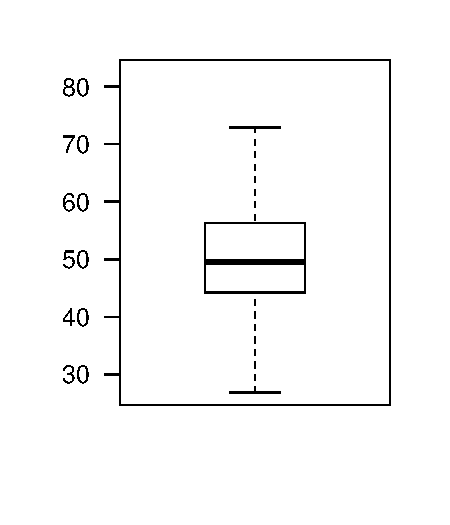
\includegraphics[scale=0.75]{C:/Users/michaelnelso/git/NRC290B/slides/slide_images/bw.pdf}};
\end{tikzpicture}

\end{frame}

\begin{frame}[fragile]{Exploratory: \emph{Box-whisker/Box plot}}

\begin{itemize}
\tightlist
\item
  \texttt{R}: \texttt{boxplot(x)}
  \texttt{\textcolor{gray}{\# x is data}}
\end{itemize}

\begin{tikzpicture}[overlay]
\node[inner sep=0pt] (one) at (5,-2.7) {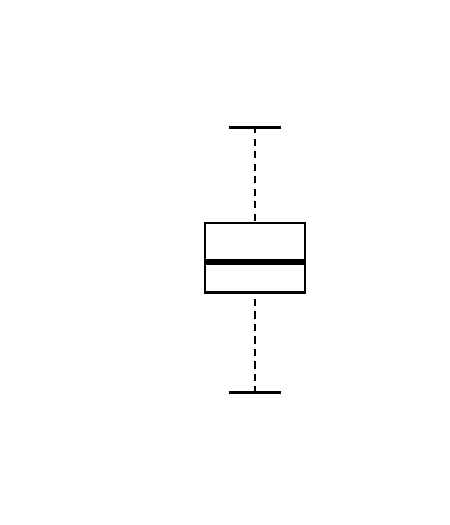
\includegraphics{C:/Users/michaelnelso/git/NRC290B/slides/slide_images/four.pdf}};
\draw[thick,blue,<-] (6.5,-2.7) -- (7.5,-2.7) node[right, black] {Median ($Q_{2}$)};
\draw[thick,blue,<-] (6.5,-2.1) -- (7.5,-2.1) node[right, black] {Upper quartile ($Q_{3}$)};
\draw[thick,blue,<-] (6.5,-3.25) -- (7.5,-3.25) node[right, black] {Lower quartile ($Q_{1}$)};
\draw[thick,blue,<->] (4.5,-3.25) -- (4.5,-2.1) node[midway, left, black, text width = 2.5cm] {Inter quartile range (IQR)};
\draw[thick,blue,<-] (5,-0.38) -- (4,-0.38) node[left, black] {Maximum};
\draw[thick,blue,<-] (5,-4.9) -- (4,-4.9) node[left, black] {Minimum};
\end{tikzpicture}

\end{frame}

\begin{frame}[fragile]{Exploratory: \emph{Line graph}}

Line graph is a useful plot for running average or time series data

\begin{Shaded}
\begin{Highlighting}[]
\KeywordTok{plot}\NormalTok{(bear.run, }\DataTypeTok{type=}\StringTok{"l"}\NormalTok{) }\CommentTok{#"l": line, "p": points, "b": both}
\KeywordTok{lines}\NormalTok{(poop.run)}
\end{Highlighting}
\end{Shaded}

\begin{tikzpicture}[remember picture,overlay]
\node[yshift=4cm] at (current page.south)
{\includegraphics[height=3in]{

```r
plot(bp$Poop, lwd = 2, col = 4, bty = "l", las = 1, ylab = "Running Average", xlab = "no. of samples", ylim = c(0,2), type = "l")
lines(bp$Bear, lwd=2, col=2, bty="l", las=1, ylab = "Running Average", xlab = "no. of samples")
abline(h = mean(bp$Bear), lty=2, col=2)
```

![](NRC290B_06_1_v4_graphical_exploration_mfn_2020_files/figure-beamer/unnamed-chunk-7-1.pdf)<!-- --> 
}};
\end{tikzpicture}

\end{frame}

\begin{frame}{Differences}

To visualize differences between groups

\begin{itemize}
\tightlist
\item
  box-whisker plots

  \begin{itemize}
  \tightlist
  \item
    compares averages
  \item
    compares distribution
  \end{itemize}
\item
  bar charts

  \begin{itemize}
  \tightlist
  \item
    compares averages
  \end{itemize}
\end{itemize}

\end{frame}

\begin{frame}[fragile]{Differences: \emph{Box-whisker plot}}

Compare salamander snout-vent lengths be three sexes:

\begin{Shaded}
\begin{Highlighting}[]
\KeywordTok{boxplot}\NormalTok{(mander}\OperatorTok{$}\NormalTok{SVL }\OperatorTok{~}\StringTok{ }\NormalTok{mander}\OperatorTok{$}\NormalTok{Sex) }\CommentTok{#formula notation}
\end{Highlighting}
\end{Shaded}

\begin{tikzpicture}[remember picture,overlay]
\node[yshift=4cm] at (current page.south)
{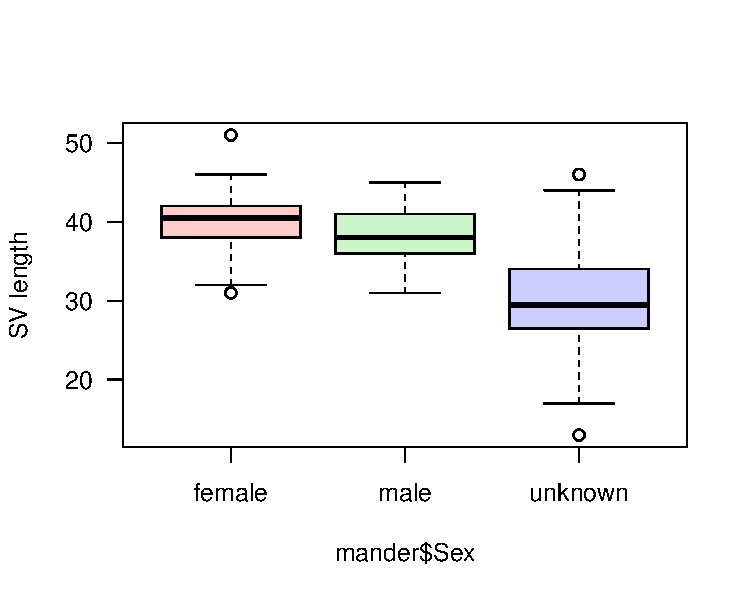
\includegraphics[height=3in]{C:/Users/michaelnelso/git/NRC290B/slides/slide_images/salbox.pdf}};
\end{tikzpicture}

\end{frame}

\begin{frame}[fragile]{Differences: \emph{Bar chart}}

Compare salamander snout-vent lengths be three sexes:

\begin{Shaded}
\begin{Highlighting}[]
\NormalTok{bars <-}\StringTok{ }\KeywordTok{tapply}\NormalTok{(mander}\OperatorTok{$}\NormalTok{SVL,mander}\OperatorTok{$}\NormalTok{Sex,mean) }\CommentTok{#create matrix (like pivot table)}
\KeywordTok{barplot}\NormalTok{(bars)                              }\CommentTok{# plot it}
\end{Highlighting}
\end{Shaded}

\begin{tikzpicture}[remember picture,overlay]
\node[yshift=4cm] at (current page.south)
{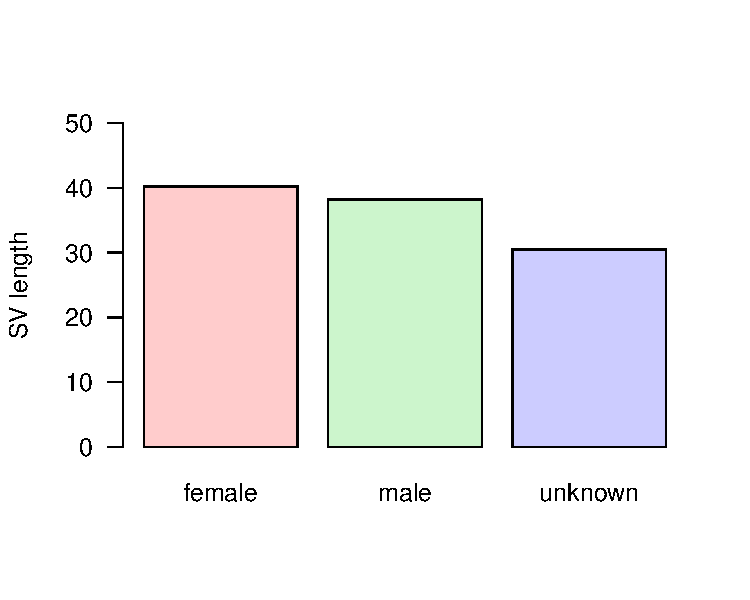
\includegraphics[height=3in]{C:/Users/michaelnelso/git/NRC290B/slides/slide_images/salbar.pdf}};
\end{tikzpicture}

\end{frame}

\begin{frame}[fragile]{Differences: \emph{Bar chart} with associated
error}

Compare salamander snout-vent lengths be three sexes:

\begin{Shaded}
\begin{Highlighting}[]
\NormalTok{bars <-}\StringTok{ }\KeywordTok{tapply}\NormalTok{(mander}\OperatorTok{$}\NormalTok{SVL,mander}\OperatorTok{$}\NormalTok{Sex,mean)}
\KeywordTok{barplot}\NormalTok{(bars)}
\end{Highlighting}
\end{Shaded}

\begin{tikzpicture}[remember picture,overlay]
\node[yshift=4cm] at (current page.south)
{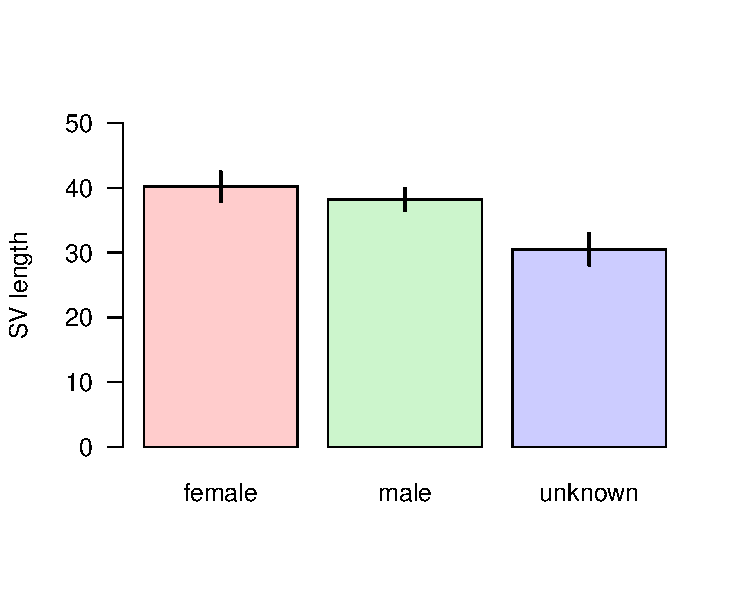
\includegraphics[height=3in]{C:/Users/michaelnelso/git/NRC290B/slides/slide_images/salbarse.pdf}};
\end{tikzpicture}

\end{frame}

\begin{frame}{Links}

Two main approaches for relationships between data:

\begin{itemize}
\item[1.]<1-> Correlations
\item[2.]<1-> Associations
\end{itemize}

\end{frame}

\begin{frame}{Links}

Two main approaches for graphing relationships between data:

\vspace{0.06cm}

\begin{itemize}
\item[1.]<1-> Correlations
  \begin{itemize}
  \item<1-> two numeric variables
    \begin{itemize}
    \item<1-> \emph{de}pendent variable (of primary interest: y-axis)
    \item<1-> \emph{inde}pendent variable (explanatory variable: x-axis)
    \end{itemize}
  \item<1-> how one variable is related to another
  \item<1-> \emph{scatter plots}
  \end{itemize}
\end{itemize}

\end{frame}

\begin{frame}[fragile]{Links: \emph{Scatter plot}}

\begin{Shaded}
\begin{Highlighting}[]
\KeywordTok{plot}\NormalTok{(x,y) }\CommentTok{# x and y are numeric vectors}
\end{Highlighting}
\end{Shaded}

\begin{tikzpicture}[remember picture,overlay]
\node[yshift=4cm] at (current page.south)
{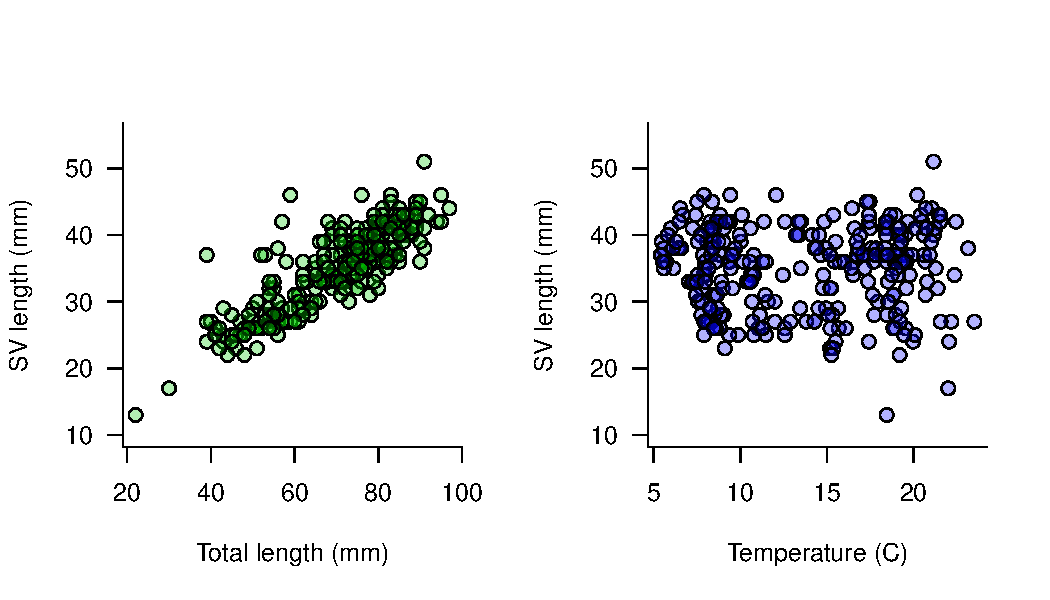
\includegraphics[height=2.5in]{C:/Users/michaelnelso/git/NRC290B/slides/slide_images/salscatter.pdf}};
\end{tikzpicture}

\end{frame}

\begin{frame}{Links}

Two main approaches for graphing relationships between data:

\begin{itemize}
\item[2.]<1-> Associations
  \begin{itemize}
  \item<1-> categorical data
  \item<1-> summarize categories
    \begin{itemize}
    \item<1-> counts
    \item<1-> proportions
    \item<1-> by rows and/or columns of a table
  \end{itemize}
  \item<1-> \emph{pie charts} for single categories 
  \item<1-> \emph{bar graphs} for several categories
  \end{itemize}
\end{itemize}

\end{frame}

\begin{frame}[fragile]{Links: \emph{Pie chart}}

\begin{Shaded}
\begin{Highlighting}[]
\NormalTok{pietab <-}\StringTok{ }\KeywordTok{table}\NormalTok{(classData}\OperatorTok{$}\NormalTok{Eyes)}
\KeywordTok{pie}\NormalTok{(pietab) }\CommentTok{#(number of people with each eye color)}
\end{Highlighting}
\end{Shaded}

\begin{tikzpicture}[remember picture,overlay]
\node[yshift=4cm] at (current page.south)
{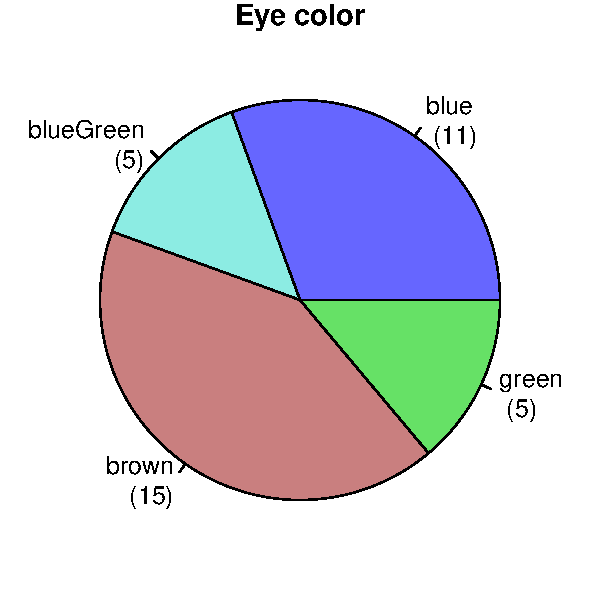
\includegraphics[height=2in]{C:/Users/michaelnelso/git/NRC290B/slides/slide_images/classpie.pdf}};
\end{tikzpicture}

\end{frame}

\begin{frame}[fragile]{Links: \emph{Bar chart}}

\begin{Shaded}
\begin{Highlighting}[]
\NormalTok{bartab <-}\StringTok{ }\KeywordTok{table}\NormalTok{(classData}\OperatorTok{$}\NormalTok{Gender,classData}\OperatorTok{$}\NormalTok{Eyes)}
\KeywordTok{barplot}\NormalTok{(pietab, }\DataTypeTok{beside=}\OtherTok{TRUE}\NormalTok{) }\CommentTok{#(number of each gender with each eye color)}
\end{Highlighting}
\end{Shaded}

\begin{tikzpicture}[remember picture,overlay]
\node[yshift=3.5cm] at (current page.south)
{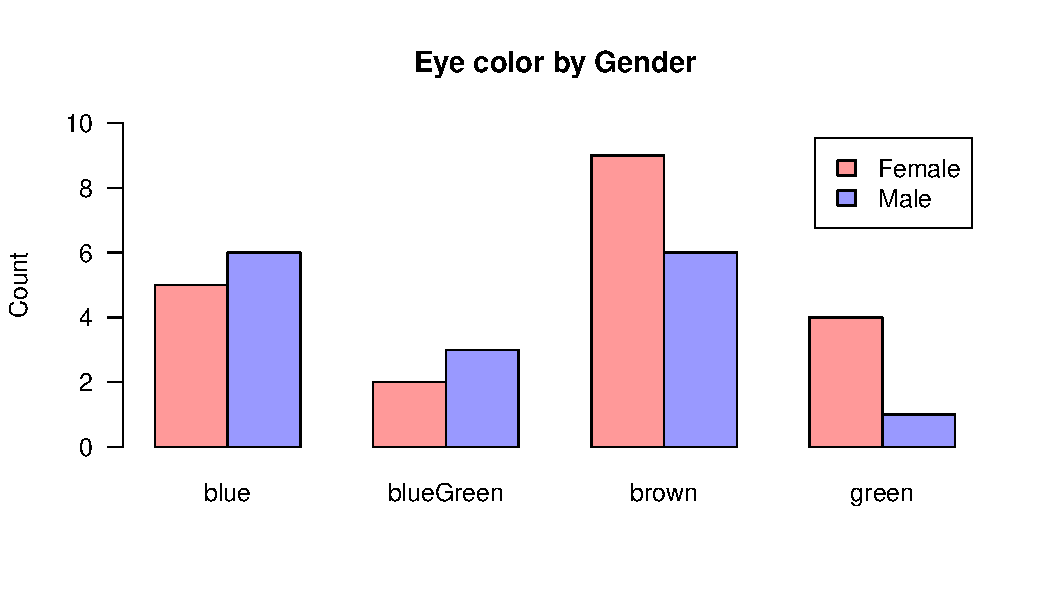
\includegraphics[height=2.5in]{C:/Users/michaelnelso/git/NRC290B/slides/slide_images/classbar.pdf}};
\end{tikzpicture}

\end{frame}

\begin{frame}{Some graphics pointers}

In summary, graphs are a useful data visualization tool

\begin{itemize}
\tightlist
\item
  summarizing
\item
  understanding
\item
  describing
\item
  presenting/communicating
\end{itemize}

\end{frame}

\begin{frame}{Some graphics pointers}

In summary, graphs are a useful data visualization tool

\begin{itemize}
\tightlist
\item
  summarizing
\item
  understanding
\item
  describing
\item
  presenting/communicating
\end{itemize}

\textbf{BUT} we must label the well or they are useless!

\begin{itemize}
\tightlist
\item
  label both axes
\item
  provide a main title for your graph
\item
  avoid clutter
\item
  make it readable
\item
  \emph{I expect graphs to be propery labeled from now on}!
\end{itemize}

\end{frame}

\begin{frame}{Some graphics pointers}

In summary, graphs are a useful data visualization tool

\vspace{1cm}

\begin{longtable}[]{@{}ll@{}}
\toprule
Purpose & Graph Type\tabularnewline
\midrule
\endhead
Illustrating \emph{distribution} & Histogram, Density
plot\tabularnewline
& Box(-whisker) plot\tabularnewline
Illustrating \emph{differences} & Bar chart, Box plot\tabularnewline
Illustrating \emph{correlations} & Scatter plot\tabularnewline
Illustrating \emph{associations} & Pie chart, Bar chart\tabularnewline
Illustrating \emph{sample size} & Line plot of running
avg\tabularnewline
\bottomrule
\end{longtable}

\end{frame}

\begin{frame}{Beyond graphs, Towards statistics}

\begin{itemize}
\item
  Graphs are powerful tools that provide insight and understanding of
  the patterns and relationships in the data.
\item
  Don't give us the answer though:

  \begin{itemize}
  \tightlist
  \item
    are differences \emph{significant}?
  \item
    are associations \emph{significatnt}?
  \end{itemize}
\end{itemize}

\begin{tikzpicture}[remember picture,overlay]
\node[yshift=3cm] at (current page.south)
{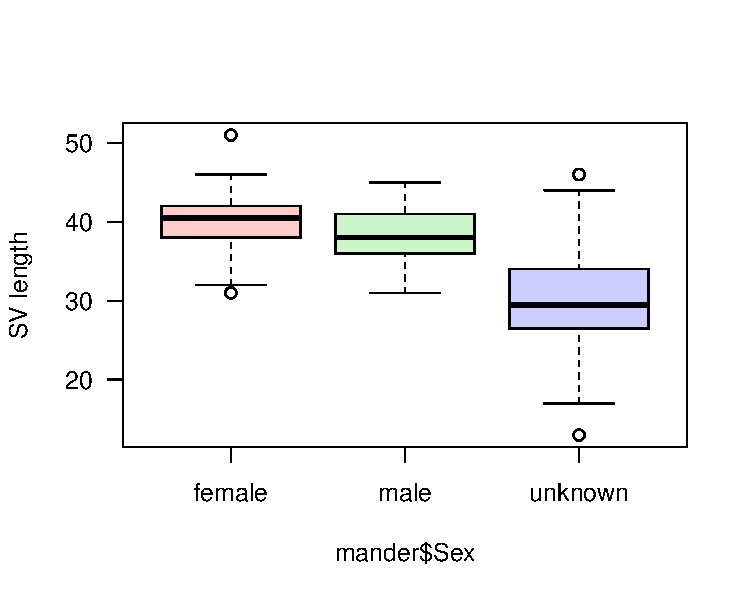
\includegraphics[height=2in]{C:/Users/michaelnelso/git/NRC290B/slides/slide_images/salbox.pdf}};
\end{tikzpicture}

\end{frame}

\begin{frame}{Beyond graphs, Towards statistics}

\begin{itemize}
\item
  Graphs are powerful tools that provide insight and understanding of
  the patterns and relationships in the data.
\item
  Don't give us the answer though:

  \begin{itemize}
  \tightlist
  \item
    are differences \emph{significant}?
  \item
    are associations \emph{significatnt}?
  \end{itemize}
\end{itemize}

\begin{tikzpicture}[remember picture,overlay]
\node[yshift=3cm] at (current page.south)
{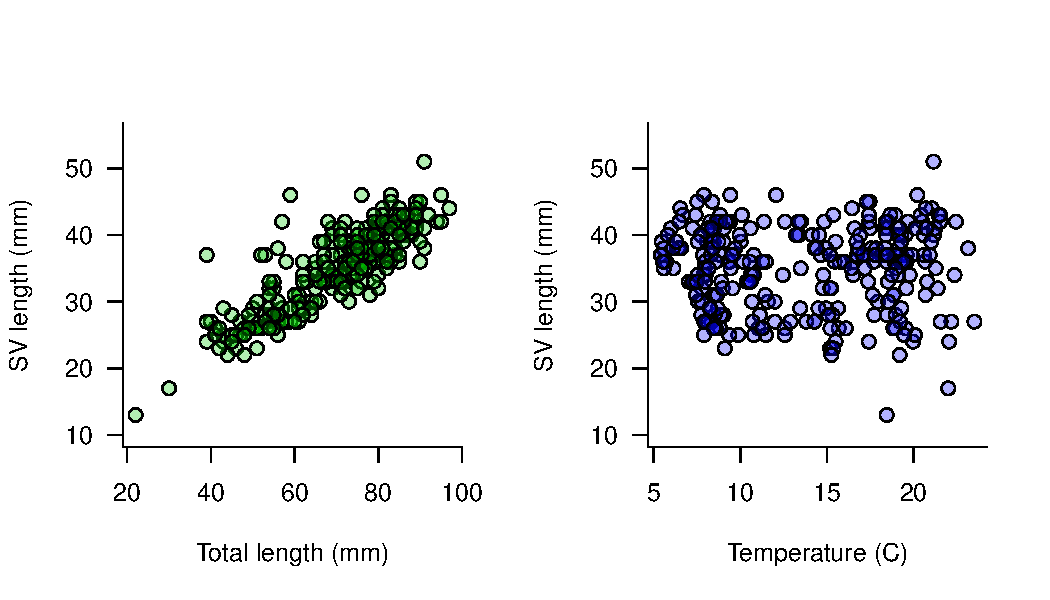
\includegraphics[height=2in]{C:/Users/michaelnelso/git/NRC290B/slides/slide_images/salscatter.pdf}};
\end{tikzpicture}

\end{frame}

\begin{frame}{Beyond graphs, Towards statistics}

\begin{itemize}
\item
  Graphs are powerful tools that provide insight and understanding of
  the patterns and relationships in the data.
\item
  Don't give us the answer though:

  \begin{itemize}
  \tightlist
  \item
    are differences \emph{significant}?
  \item
    are associations \emph{significatnt}?
  \end{itemize}
\item
  Statistics is the tool we use to formally answer these questions!

  \begin{itemize}
  \tightlist
  \item
    the differences \emph{are}/\emph{are not} significant!
  \item
    are associations \emph{are}/\emph{are not} significant!
  \end{itemize}
\end{itemize}

\end{frame}

\end{document}
